\chapter{方案模型}
本章将系统性介绍本文提出的可验证区块链查询方案的整体架构、数据与查询建模、核心算法流程及安全性目标。通过形式化建模与安全分析，为后续方案实现与性能评估奠定理论基础。

\section{系统模型}
本文提出了一种新的vscc框架，研究了在密态区块链数据库上的可验证查询处理。如图\ref{fig:system-model}展示了本文的系统模型。
DO 负责系统初始化、数据加密、索引构建与更新，并将密文索引上传至区块链，而真实数据以加密形式存储在链下数据库中。DU 作为轻量级节点，在本地利用授权密钥材料生成查询陷门，
并向 SP 发起查询请求。SP 基于链上索引执行检索，生成结果集及验证对象后广播给其他全节点进行共识投票。投票结果同时记录在区块链上，以支持结果审计和抗抵赖。
最终，SP 将带有共识签名的查询结果返回给 DU，DU 在本地完成验证与解密。

\begin{figure}[h]
    \centering
    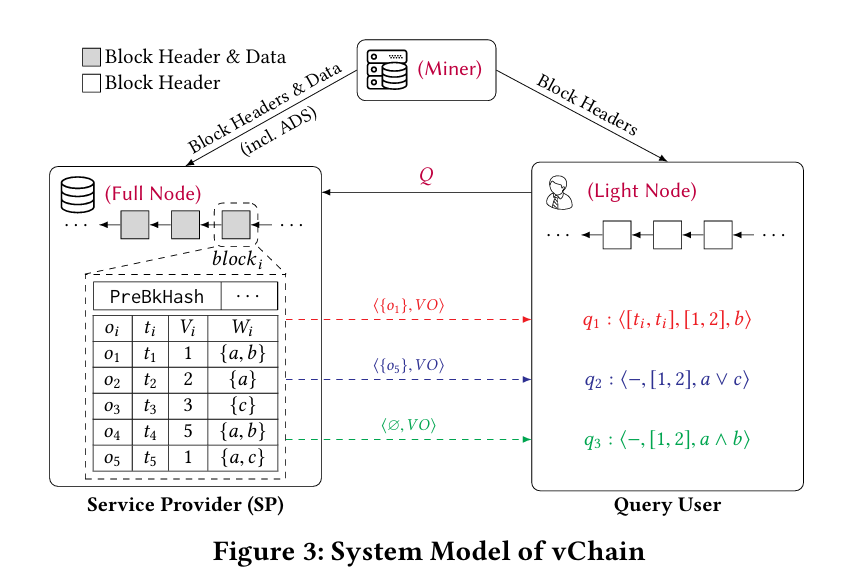
\includegraphics[width=0.5\textwidth]{figures/System-Model-of-vscc.png}
    \caption{vChain系统模型}
    \label{fig:system-model}
\end{figure}

为了实现对存储在区块链或分布式数据库中复杂数据的统一处理，我们对数据对象及用户查询请求进行形式化建模。

我们将系统中的数据对象建模为一系列序列化对象$o_1, o_2, \dots, o_n$，每个数据对象 $o_i$ 都可以表示为三元组:
\begin{equation}
    o_i = \langle T_i,V_i,W_i \rangle
\end{equation}

其中，$T_i$ 表示对象的时间属性，在本文场景下可等同理解为对象写入时对应的区块高度；$V_i$ 表示对象的数值属性向量，为了便于说明，下文主要以一维数值属性为例；$W_i$ 表示对象的关键字集合。例如，考虑一条供应链金融中的资产凭证记录 $o_i = \langle 2024 \text{-} 03 \text{-} 22 ; 10:00:00,; 5000,; {\text{“Alice”},\text{“Bob”}} \rangle$。该对象包括一个交易时间戳 $T_i = 2024 \text{-} 03 \text{-} 22 ; 10:00:00$，属性值集合 $V_i$ 记录了该笔资产的金额 $5000$ 元，而 $W_i$ 则包含了该资产的发行方“Alice”、接收方“Bob”。

基于上述建模，用户发起的复杂检索请求可以表示为一个三元组查询：
\begin{equation}
    Q = \langle [t_s,t_e],\Phi_{W},\Phi_{V}\rangle
\end{equation}

其中，$[t_s, t_e]$ 是查询时间区间，$\Phi_{W}$ 为定义在关键字上的布尔表达式，仅支持合取与析取，$\Phi_{V}$ 为定义在数值属性上的范围查询。当查询不包含某类条件时，可将对应谓词记为空。
例如，一个典型的审计查询可以表示为：$Q = \langle [2024\text{-}01, 2024\text{-}03],; [1000, 5000],; (\text{Buyer: Alice} \wedge \text{Status: Approved}) \rangle$。该查询将搜索所有时间戳在 2024 年第一季度内、金额位于 $[1000, 5000]$ 范围内，且属性同时满足买方为 Alice 和状态为“已审核”的交易记录。

由于系统采用滑动窗口模型，每个区块仅承诺以该块为右端点的当前窗口状态，因此针对时间区间$[t_s,t_e]$的查询，需要被划分为一组与时间窗口状态对齐的子查询，每个子查询都对应某个窗口末端区块上的索引根，从而保证查询、验证与链上状态严格对应。

\section{系统形式化定义}
本文提出的可验证查询方案由以下六个多项式时间算法组成：

（1）\quad $\textsf{Setup}(1^\lambda) \to (msk, params)$：由数据拥有者（DO）执行。输入安全参数 $\lambda$，输出系统主密钥 $msk$（包含对称密钥 $mk$ 和累加器私钥 $sk$）及公开参数 $params$（包含累加器公钥 $pk$ 和全局注册表配置）。

（2）\quad $\textsf{GenIndex}(D, msk) \to (I, acc)$：由 DO 执行。输入原始数据集 $D$，利用 $msk$ 对数据进行预处理、规范化及加密映射，生成密文索引 $I$（即 \texttt{IndexedObject}）和对应的累加器摘要 $acc$。

（3）\quad $\textsf{Trapdoor}(Q, msk) \to T_Q$：由数据用户（DU）执行。输入查询请求 $Q = \langle [t_s, t_e], [a, b], \phi \rangle$，利用授权密钥材料生成包含密文令牌（Tokens）的查询陷门 $T_Q$ 。

（4）\quad $\textsf{Query}(I, T_Q, params) \to (R, \pi)$：由服务提供商（SP）执行。SP 在密文索引 $I$ 上检索满足陷门 $T_Q$ 条件的结果集 $R$，并根据集合运算逻辑生成对应的密码学证明 $\pi$。

（5）\quad $\textsf{Verify}(R, \pi, params, acc) \to \{0, 1\}$：由 DU 或全节点执行。利用公开参数和累加器摘要验证结果集 $R$ 的可靠性与完整性。若验证通过则输出 $1$，否则输出 $0$。

（6）\quad $\textsf{Decrypt}(R, msk) \to D_R$ ：由 DU 执行。对通过验证的结果集进行解密，恢复出原始明文数据。
\begin{table}[htbp]
	\centering
	\caption{方案主要符号及其含义}
	\label{tab:notations}
	\begin{tabular}{@{} l l l @{}}
		\toprule
		符号 & 含义说明 \\
		\midrule
		$\lambda$ & 系统安全参数 \\
		$mk$ & 对称主密钥 (Master Key) \\
		$sk, pk$ & 累加器私钥与公钥 \\
		$O_i$ & 第 $i$ 个原始数据对象 \\
		$IO_i$ & 密文索引对象 (Indexed Object) \\
		$acc(X)$ & 集合 $X$ 的累加器摘要值 \\
		$Token$ & 加密令牌 (Token) \\
		$ID_{kw}, ID_{pf}$ & 注册表编号 \\
		$P_X(z)$ & 特征多项式 \\
		$T_Q$ & 查询陷门 (Trapdoor) \\
		$\pi_{opt}$ & 集合运算证明 (Proof) \\
		$e(\cdot, \cdot)$ & 双线性配对运算 \\
		\bottomrule
	\end{tabular}
\end{table}
\section{威胁模型与安全目标}

\subsection{安全模型}
本方案的安全性通过攻击者 $\mathcal{A}$ 与挑战者 $\mathcal{B}$ 之间的形式化博弈进行定义。
\subsubsection{关键字猜测攻击安全博弈}
由于本方案中的关键字令牌 $Token_{kw}$ 存储在公开的注册表中，必须证明即使敌手获知部分令牌和对应的索引 ID，也无法在离线状态下通过枚举关键字来识别未知的陷门。

初始化 (Setup)：挑战者 $\mathcal{B}$ 运行密钥生成算法，生成主密钥 $mk$ 和累加器参数 $(pk, sk)$。$\mathcal{B}$ 将安全参数 $\lambda$ 和公钥 $pk$ 发送给敌手 $\mathcal{A}$。

陷门询问 (Trapdoor Query)：$\mathcal{A}$ 适应性地选择关键词集合 $W$ 提交给 $\mathcal{B}$。$\mathcal{B}$ 返回由 $mk$ 加密生成的令牌集合 $T_W = \{F(mk, kw) \mid kw \in W\}$。

挑战 (Challenge)：$\mathcal{A}$ 选择两个从未被询问过且等长的目标关键词集 $W_0^*$ 和 $W_1^*$ 提交。$\mathcal{B}$ 随机选择 $b \in \{0,1\}$，计算挑战索引 $I_b^*$ 并发送给 $\mathcal{A}$。

猜测 (Guess)：$\mathcal{A}$ 输出猜测值 $b' \in \{0, 1\}$。如果 $b' = b$，则称 $\mathcal{A}$ 赢得博弈。

安全定义：若对于任何多项式时间敌手 $\mathcal{A}$，其赢得游戏的优势 $\mathrm{Adv}_{\mathcal{A}}^{\mathrm{KGA}}(\lambda) = |\mathrm{Pr}[b'=b] - 1/2|$ 是可忽略的，则称方案满足抗关键词猜测攻击安全性。
\subsubsection{密文不可区分性}
为了证明非对称累加器部分的安全性，我们参考经典的 IND-CKA (Chosen-Keyword Attack) 模型。该模型确保了累加器摘要 $AccValue$ 不会泄露其包含的特定特征 ID 的任何代数信息

Setup：$\mathcal{B}$ 生成累加器公私钥对 $(pk, sk)$ 并将 $pk$ 发送给 $\mathcal{A}$。

Interrogation：$\mathcal{A}$ 提交多个集合 $S_i$，$\mathcal{B}$ 返回对应的累加器摘要 $acc(S_i) = g^{P_{S_i}(s)}$。

Challenge：$\mathcal{A}$ 选取两个不同但基数相同的集合 $S_0^*, S_1^*$。$\mathcal{B}$ 随机选取 $b \in \{0, 1\}$ 并返回挑战摘要 $acc(S_b^*)$。

Guess：$\mathcal{A}$ 输出猜测 $b'$。

安全定义：该安全性归约至双线性群上的 $q$-强 Diffie-Hellman ($q$-SDH) 困难性假设。在 $q$-SDH 假设成立的前提下，$\mathcal{A}$ 无法以不可忽略的优势区分两个不同集合的累加结果。


\subsection{安全目标}
在本方案中中的分布式架构中，信任边界仅存在于数据拥有者（DO）与本地存储之间，外部实体均被视为潜在的对手。
SP 负责托管密文索引并执行检索计算。由于程序故障、恶意攻击或商业利益驱动（如减少算力开销），SP 被认为是非诚实的。它可能
修改存储的对象内容或伪造不存在的对象，也可能在复杂的集合运算（交、并、差）中遗漏部分符合条件的子集。
在分布式交易或审计场景中，DU 可能会发起抵赖攻击（Repudiation Attack）。
当 DU 接收到正确的查询结果后，为了逃避服务付费或恶意诬陷 SP，DU 可能会否认收到过正确的结果，
声称 SP 提供的证明 $\pi_{opt}$ 无效或数据不完整。针对上述复杂的威胁环境，本方案旨在实现以下详尽的安全目标：

（1）\quad \textbf{完整性（Integrity）：} 确保 SP 无法篡改存储的对象内容或伪造不存在的对象。任何对存储对象的修改都必须被 DU 发现。

（2）\quad \textbf{正确性（Correctness）：} 确保 SP 在执行集合运算（交、并、差）时，返回的结果集必须完全包含所有满足查询条件的对象，且不包含任何不满足条件的对象。

（3）\quad \textbf{抗抵赖性（Non-repudiation）：} 确保 DU 无法否认收到过正确的查询结果。任何 DU 的抵赖行为都应被系统记录并可供审计。


\subsection{本章小结}
\\这里AI率很高
本章围绕可验证区块链查询方案，系统阐述了系统模型、数据与查询建模、核心算法流程及安全性目标。
通过形式化定义与安全博弈分析，明确了各参与方的职责与潜在威胁，并提出了完整性、正确性和抗抵赖等关键安全目标。
这些内容为后续方案实现、优化与性能评估提供了理论基础和设计依据。

